
\subsection{Application performance -- memcache}
\label{sec:eval:memcached}



\begin{figure}
\centering    \includegraphics{figs/connscaling-throughput.eps}
\caption{Throughput for varying established connections}
\label{fig:connscaling}
\end{figure}

\begin{figure*}
\begin{centering}
\subfloat[Multilate-Me !]{
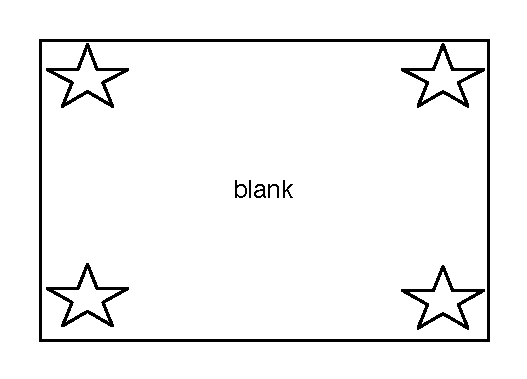
\includegraphics[width=3.1in]{figs/blank.eps}}
\subfloat[Multilate-Me Again!]{
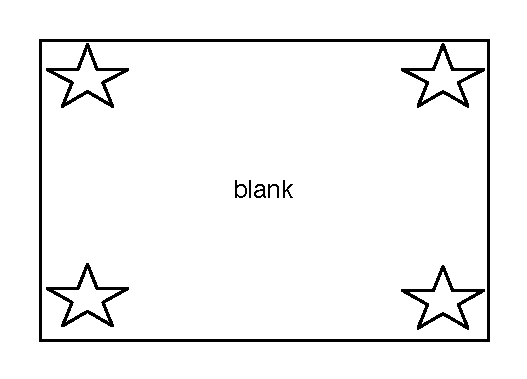
\includegraphics{figs/blank.eps}}
\caption{Capacity and quality of service of memcached on Linux and \ix for XXX and YYY concurrent, established connections}
\label{fig:mutilate}
\end{centering}
\end{figure*}



We now validate the performance benefits of the protected dataplane
design on memcached -- a real world, massively deployed, in-memory
key-value store built on top of the libevent framework.  We use the
mutilate~\cite{url:mutilate} load-generator to measure median and 95th
percentile latency as a function of the throughput delivered by the
server~\cite{Leverich:RHSU:2014}. 

Fig.~\ref{fig:mutilate} reports the latencies as a function of the
number of queries per second for synthetic workloads modelled after
Facebook's \texttt{ETC} and \texttt{USR} workloads~\cite{Atikoglu:2012:WAL}.

\edb{PLACEHOLDER} The peak QPS is measured using \ix at
XXX, which maps to a bandwidth leaving the server of XXX Gbps, or XX\%
of the theoretical wire rate of the machine.  We report the numbers
for Linux and \ix for XXX and YYY established, concurrent
connections served by the 18 clients.

Our results show that \edb{TODO}.....


%
\subsection{Multi-tier Performance}

\edb{THIS IS A STRECH STRETCH GOAL} 

Evaluating the performance of a highly-scalable, multi-tier
environment in a lab environment is challenging on multiple fronts:
first, there are ---to the best of our knowledge--- no universally
accepted multi-tier benchmarks that involve key-value stores and in
general that are representative of web-scale applications.  Second,
most lab enviornments are orders of magnitude smaller than a
datacenter.

Therefore, we construct a simple, synthetic multi-tier benchmark that
mimics the behavior of a social application stored in an in-memory
key-value store.  The application is a simple \texttt{http} server
that returns the top-most recent update among a users list of friends.
The application server parses the http request to
get the userid, uses the user id to return a friends-list from a
key-value store, and then queries the key-value store individually for
each friend for the most recent value.  It then processes replies and
return the top-most entries.  In our experiments, we model a database
with $10^7$ million users, each with 100 friends. 

We scale the benchmark to model a cluster deployment with $\alpha$
client connections per application server, $\beta$ httpd and $\gamma$
memcached servers.  Keys are distributed uniformly between the
$\gamma$ servers.  We model a large-scale deployment with
$\alpha=10^5$, $\beta=10^4$ and $\gamma=10^4$ on a deployment that consists of 4
actual application servers and 1 memcached server (running on our
server hardware with 4x10GbE connectivity).  Each application server
runs \texttt{lighthttpd} with the application logic written directly
within the server, and maintains a distinct connection for each of the
$\alpha$ virtual clients and $\gamma$ virtual nodes.  The key-value store is
running \texttt{memcache} as described in \S\ref{sec:eval:memcache}.
We use the remaining 14 client machines to simulate $4 \times \alpha$
clients and the 19th client to measure the latency of the application.

Fig.~\ref{missing} reports the latency as a function of the
throughput, as determined by varying the client load.  We compare a
Linux baseline with one in which \ix is used to run both the
application server and the memcached server.  We note that the choice
of operating system on the application server determines the number of
concurrent connections. Indeed, because of the coherence-free
execution model, each application server needs to open a distinct TCP
flow to the same virtual node for each of its hardware threads.

\edb{OPTIMISTIC: } Fig.~\ref{missing} shows that \ix can saturate the
hardware connectivity.  Indeed, the bottlneck consits of the
communication 





